\documentclass[onecolumn, draftclsnofoot,10pt, compsoc]{IEEEtran}
\usepackage{graphicx}
\usepackage{url}
\usepackage{setspace}
\usepackage[usenames,dvipsnames,svgnames,table]{xcolor}

\usepackage{geometry}
\geometry{textheight=9.5in, textwidth=7in}

% 1. Fill in these details
\def \CapstoneTeamName{		GROUP65}
\def \CapstoneTeamNumber{		65}
\def \GroupMemberOne{			Jacob Geddings}
\def \GroupMemberTwo{			Inhyuk Lee}
\def \GroupMemberThree{			Juan Mugica}
\def \CapstoneProjectName{		CDK Data Stream AI}
\def \CapstoneSponsorCompany{	CDK Global}
\def \CapstoneSponsorPerson{		Chris Smith}

% 2. Uncomment the appropriate line below so that the document type works
\def \DocType{		Problem Statement
				%Requirements Document
				%Technology Review
				%Design Document
				%Progress Report
				}
			
\newcommand{\NameSigPair}[1]{\par
\makebox[2.75in][r]{#1} \hfil 	\makebox[3.25in]{\makebox[2.25in]{\hrulefill} \hfill		\makebox[.75in]{\hrulefill}}
\par\vspace{-12pt} \textit{\tiny\noindent
\makebox[2.75in]{} \hfil		\makebox[3.25in]{\makebox[2.25in][r]{Signature} \hfill	\makebox[.75in][r]{Date}}}}
% 3. If the document is not to be signed, uncomment the RENEWcommand below
%\renewcommand{\NameSigPair}[1]{#1}

%%%%%%%%%%%%%%%%%%%%%%%%%%%%%%%%%%%%%%%
\begin{document}
\begin{titlepage}
    \pagenumbering{gobble}
    \begin{singlespace}
    	\includegraphics[height=4cm]{coe_v_spot1}
        \hfill 
        % 4. If you have a logo, use this includegraphics command to put it on the coversheet.
        %\includegraphics[height=4cm]{CompanyLogo}   
        \par\vspace{.2in}
        \centering
        \scshape{
            \huge CS Capstone \DocType \par
            {\large\today}\par
            \vspace{.5in}
            \textbf{\Huge\CapstoneProjectName}\par
            \vfill
            {\large Prepared for}\par
            \Huge \CapstoneSponsorCompany\par
            \vspace{5pt}
            {\Large\NameSigPair{\CapstoneSponsorPerson}\par}
            {\large Prepared by }\par
            Group\CapstoneTeamNumber\par
            % 5. comment out the line below this one if you do not wish to name your team
            %\CapstoneTeamName\par 
            \vspace{5pt}
            {\Large
                \NameSigPair{\GroupMemberOne}\par
                \NameSigPair{\GroupMemberTwo}\par
                \NameSigPair{\GroupMemberThree}\par
            }
            \vspace{20pt}
        }
        \begin{abstract}
        % 6. Fill in your abstract    
		Our team has been assigned to assist in the development of AI for application to CDK’s existing Data Streams. 
		The goal in doing this is to gain insight from said data streams, use this data to predict future events, and detect when an anomaly is present. 
		These three goals need to be independent of one another and be capable of functioning as a black box. 
		This entails the ability to write applications and/or functions that are then fed through the system in various ways. 
		Tools that will be necessary for project completion include the AWS platform, Docker, Linux platform, and several open source AI resources.	
        \end{abstract}     
    \end{singlespace}
\end{titlepage}
\newpage
\pagenumbering{arabic}
\tableofcontents
% 7. uncomment this (if applicable). Consider adding a page break.
%\listoffigures
%\listoftables
\clearpage

% 8. now you write!
\section{The Problem}
	ROUGH DRAFT PRE-MEETING WITH CLIENT
The Problem:
CDK is a company focused in automotive dealership that has affiliated offices around the world each providing their own personal design regarding documentation as well as dealing with unique laws of the various countries they reside in. Given the diverse nature of this setup CDK is in a difficult spot with the gathering, documenting, and proofreading of these documents. Adding to this issue is the fact that these documents are physical and need to be scanned in for safe storage which leads to concerns regarding consistency. Some concerns are: differing file extensions, scanning errors, and physical damage of the document. As it stands it is too easy for errors to slip through and is too costly to locally check each document as they have done in the past. 

\section{Solution and Rules}
Solution and Rules:
With this challenge CDK has proposed a solution, a single AI platform that can process digitally submitted documents with the intent of confirming whether a document has been signed. This proposition comes with a few hard-line rules that must be followed. These rules are: use of an open source AI, follow a black box design, and formatted in such a way that a new team can take over after project completion. Failure is a recognized possibility and should failure occur a detailed write up as to the what, where, and why of the failure must be given so that CDK can either wait for the technology to meet its ambitions or explore a new approach to the problem.

\section{Primary Requirement}

The primary objective for our team is the creation of a program that can parse through images in PDF format and determine a few key points about a given document. We must be able to determine if a document was correctly signed. From this we must also confirm all signature blocks have been filled out within a form. Consideration for cosigners must also be made, prompt the user if a cosigner field is left blank for instance. CDK is also interested in detecting valid driver licenses, an example would be to check if the license has expired.
For completion of this task an AI platform will need to be selected that will best fit our needs. As it stands OpenCV is the primary candidate for completing this task but should it prove incapable two backup platforms are being considered which are DL4j and TensorFlow. OpenCV looks to be a solid choice given its numerous publicly available tutorials and guides on image processing. Its ability to readily convert images into binary coloring, line detection, and template matching will all likely be utilized for signature detection.

 The program is to be deployed on many different machines, making it essential that it be compatible with cross platform container software such as Docker. Given that the software is to learn from a large number of data points that will be provided by our client, it is also essential that it be able to run without problems for extended amounts of time. The software must be coded with scalability in mind; It should keep track of previously parsed documents and be able to consistently classify new documents into the aforementioned categories (fully signed, lacking signatures, lacking space for a signature / not applicable). 

\pagebreak

\section{Stretch Goals}
	
	Once the software can perform ALL of the aforementioned tasks with an industry satisfactory success rate (>95\% classification success rate), our client is interested in expanding the software to outline key features pertaining to pictures of vehicles clients send in. These include but are not limited to :
\begin{description}
	\item[--]The model of the vehicle.
	\item[--]The make of the vehicle .
	\item[--]License plate information.
	\item[--]Legal information regarding such licenses.
	\item[--]The condition of the vehicle: dents, cracks and scratches.
\end{description}

Given that this is a stretch goal, our client put extra emphasis on taking it one feature at a time. These features are outlined in a manner where they each provide a level of significance to the overall project .The software must first be able to detect that the picture is of a car.  Once it can satisfactorily do this (again, ~85\% classification success rate), we may move on to the next feature: detecting the license plate, and parsing it into machine readable text. If we are able to achieve a satisfactory rate in this aspect, we are then tasked to move on to detecting the make and model of the vehicle. Lastly, if all other milestones have been successfully completed, we are tasked with detecting key features regarding the vehicle's condition. 

\section{Gantt Chart}

This section details the groups schedule in complete the given tasks per the school year of 2017. Included is a Gantt chart detailing what the specific task is and the time frame over which they're scheduled to take place.

Fall Term
\begin{description}
	\item[Week 6:]10/29
	\item[End:]   Friday, December 8, 2017
\end{description}


Winter term
\begin{description}
	\item[Begin:]Monday, January 8, 2018
	\item[End:]	 Friday, March 23, 2018
\end{description}


Spring Term
\begin{description}
	\item[Begin:]Monday, April 2, 2018
	\item[Expo:] 	Tentatively May 18, 2018
	\item[End:]			Friday, June 15, 2018
\end{description}



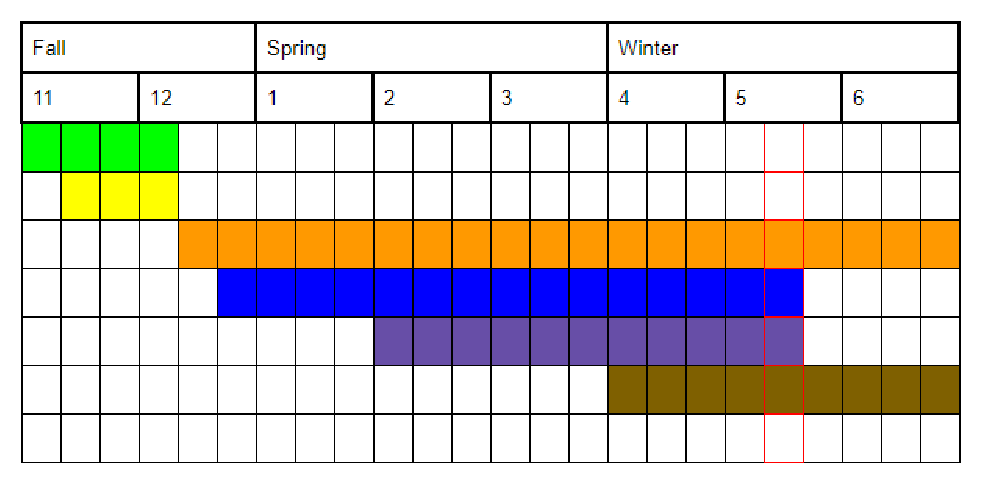
\includegraphics[height=8cm]{Gantt}


Practice
\begin{description}
	\color{green}
	\item[--]Study machine learning framework
	\color{yellow}
	\item[--]Build Small texture detecting program
\end{description}

\color{black}
Main: Build first prototype
\begin{description}
	\color{Orange}
	\item[--]Study on texture detecting A.I. algorithm
	\color{blue}
	\item[--]Build program that detects handwritten signatures from document
	\color{purple}
	\item[--]Adapt program to accept ranging document formats
	\begin{description}
		\color{black}
		\item[--]Data feeding
		\item[--]Check License information
		\item[--]Check permit information
	\end{description}
	\color{brown}
	\item[--]Optimize the program
	\begin{description}
		\color{black}
		\item[--]Debugging
	\end{description}
\end{description}
Stretch Goals (to be scheduled after completion of original goals)
\begin{description}
	\item[--]Detect the model of a vehicle
	\item[--]Detect the make of a vehicle
	\item[--]Detect/read license plate information
	\item[--]Detect/read license and permit information
	\item[--]Gather information of the condition of the vehicle (e.g.: dents, cracks and scratches)
\end{description}
\end{document}